\documentclass[10pt]{article}
\usepackage[dvipsnames]{xcolor}
\usepackage{tikz}
\usepackage{url}
\usepackage{multicol}
\usepackage{xspace}
\usepackage{pstricks}
\usepackage{wrapfig}
\usepackage[section]{placeins}
\usepackage{wrapfig}
\usepackage{listings}
\usepackage[default]{droidserif}
\usepackage[T1]{fontenc}

%\usepackage{algorithm2e}
\usetikzlibrary{arrows,automata,shapes,positioning}
\tikzstyle{block} = [rectangle, draw, fill=blue!20, 
    text width=2.5em, text centered, rounded corners, minimum height=2em]
\tikzstyle{bw} = [rectangle, draw, fill=blue!20, 
    text width=4em, text centered, rounded corners, minimum height=2em]

\newcommand{\handout}[5]{
  \noindent
  \begin{center}
  \framebox{
    \vbox{
      \hbox to 5.78in { {\bf ECE155: Engineering Design with Embedded Systems } \hfill #2 }
      \vspace{4mm}
      \hbox to 5.78in { {\Large \hfill #5  \hfill} }
      \vspace{2mm}
      \hbox to 5.78in { {\em #3 \hfill #4} }
    }
  }
  \end{center}
  \vspace*{4mm}
}

\newcommand{\lecture}[4]{\handout{#1}{#2}{#3}{#4}{Lab #1}}
\topmargin 0pt
\advance \topmargin by -\headheight
\advance \topmargin by -\headsep
\textheight 8.9in
\oddsidemargin 0pt
\evensidemargin \oddsidemargin
\marginparwidth 0.5in
\textwidth 6.5in

\parindent 0in
\parskip 1.5ex
%\renewcommand{\baselinestretch}{1.25}

\newcommand{\todo}[1]{{\red\textbf{TODO: }#1}\xspace}

\lstset{language=java, 
        basicstyle=\ttfamily,columns=fullflexible,
%	keywordstyle=\color{Blue},          % keyword style
%	commentstyle=\color{OliveGreen}\textit,       % comment style
%	identifierstyle=\color{Black},
%	stringstyle=\color{BrickRed},
	mathescape=true,
	tabsize=3,
	showstringspaces=false}

\begin{document}

\lecture{2 (Detecting Footsteps)}{Winter 2015}{Kirill Morozov}{version 1.1}

{ \bf Deadline:} You must submit the lab to the SVN repository by the submission deadline (see the syllabus) and be
prepared to demonstrate Lab 2 to a TA at the start of your assigned
Lab 3 session.  The best way to demo is during a lab session, but any
earlier time where you can convince a TA to watch is OK too.

{\bf Note:} We've deliberately made Lab 2 much less directed than Lab 1. We believe that we've included all of the background information you need. But implementation decisions are up to you.

\section{Objective}
The goal of this lab is to interpret sensor data. You will create a pedometer application for your Android phone. Your application will read the phone's accelerometer to count the user's steps. You may choose how the user will hold the phone during the demonstration. (A phone held in the user's hand will produce very different acceleration data from a phone stored in the user's pocket, or strapped to the user's shoe.) Your goal is to make your pedometer as accurate as possible.

During this lab, you will have an opportunity to:
\begin{enumerate}
\item Study accelerometer readings to identify patterns.
\item Implement more sophisticated event handlers for the accelerometer sensor.
\item Filter raw sensor data to account for noise and bias.
\item Design and implement a pedometer algorithm.
\end{enumerate}

\section{Background}

This lab builds on what you learned in Lab 1. We assume that you now know how to read the sensors on an Android phone. Most students will probably start with their Lab 1 code as a template.

But that said - don't just overwrite your lab 1. Make a new project. Check Learn for the instructions about how to copy an Eclipse project.

Here are a few hints.
\begin{enumerate}
\item You may want to use the {\tt TYPE\_LINEAR\_ACCELERATION} virtual sensor from Android. That sensor filters out gravity, while {\tt TYPE\_ACCELEROMETER} gives raw data. You might also consider registering your listener with {\tt SENSOR\_DELAY\_FASTEST} to get more sensor readings.
\item Accelerometers are noisy. You'll need to differentiate noise from data. Start by looking at the graph of the acceleration readings you get from taking ten steps. Try to see which parts of the data correspond to steps and which parts don't belong. Then try to eliminate the noise.
%% \item You will notice that, even when at rest, the accelerometer does not actually read zero for any of its axes, even after you account for the normal force. This source of error is not so important for Lab 2, since you will be looking at changes in acceleration, rather than absolute values. However, you will want to account for this bias in Lab 3.
%% \item While you can decide how the user (TA) holds the accelerometer, you do not get to decide the orientation of the phone; the TA may hold your phone upside down, for instance. There are a number of ways to solve this problem and finding one will be up to you.
\item You need to detect acceleration patterns corresponding to walking. One option is to use a simple state machine, which can work well enough for full marks. State machines also occur in ECE124; we'll review them here. More sophisticated solutions include multiple cooperating state machines. If you want more challenge after implementing state-machine-based solutions, consider a neural network for bonus marks. We're not going to say anything about those.
\item This manual will introduce you to high-pass filters, low-pass filters and finite state machines. You may find these constructs helpful, but you are free to use them or ignore them as you think best. There are many ways to correctly implement this lab. (Not all staff implementations of Lab 2 use explicit finite state machines. We strongly recommend thinking about the problem in terms of an FSM, but you don't actually need to implement a full FSM.)
\item Tired of losing your step counts on phone rotation? Implement {\tt onSaveInstanceState()}. (Not required.)
% TODO add more to the background

\end{enumerate}

\section{High and low pass filters}

\begin{figure}[ht]
\begin{center}
\includegraphics[width=0.9\textwidth]{Filters-example.png}
\end{center}
\caption{\label{fig:Filters}High-pass and low-pass filters applied to input data.}
\end{figure}

We'll introduce two mathematical constructs that you may find useful. These filters come from electronics and signal processing. A high pass filter works by attenuating low frequency signals, while a low pass filter attenuates high frequency signals. 

Consider an AM radio
signal\footnote{\url{http://en.wikipedia.org/wiki/Amplitude_modulation}}. Applying a high-pass
filter to the signal will leave us with the carrier wave while
applying a low-pass filter will eliminate the carrier wave and leave
us with the data.
Figure~\ref{fig:Filters} shows what happens when you apply a high-pass and a low-pass filter to some input data. In this case, the data series `x' is a sum of the function $f(x)=10$ and some random noise. After a few samples, the data series `high-x' closely follows the noise, while the data series `low-x' more closely approximates the constant value 10.

\newpage
\subsection{High-pass filter algorithm}
\lstset{language=java, 
	keywordstyle=\color{Blue},          % keyword style
	commentstyle=\color{OliveGreen}\textit,       % comment style
	identifierstyle=\color{Black},
	stringstyle=\color{BrickRed},
	mathescape=true}
\begin{lstlisting}[frame=trbl]{}
// Credit: http://en.wikipedia.org/wiki/Highpass_filter
float[] highpass(float[] in, float dt, float RC) {
	float[] out = new float[in.length];
	float $\alpha$ = RC / (dt + RC);
	out[0] = 0;
	for(int i = 1; i < in.length; i++) {
		out[i] = $\alpha$ * out[i-1] + $\alpha$ * (in[i] - in[i-1]);
	}
	return out;
}
\end{lstlisting}

In this implementation, $\alpha$ is to be derived from the duration between samples and a time constant. The time constant determines which frequencies are attenuated and which ones are left unchanged. Its name comes from the product of the resistance (R) and capacitance (C) used in the equivalent electric circuit implementing this high-pass filter.

A large $\alpha$ means that the filtered data series will decay slowly and be more sensitive to changes in the input. From a physical point of view, the larger the $\alpha$, the lower the frequency of signals that are attenuated. Conversely, the smaller the $\alpha$, the higher the frequency of attenuated signals. 

Since the {\tt dt} and {\tt RC} values are constant, you don't need to calculate them; you can simply choose an $\alpha$ value you find appropriate. 

\subsection{Low-pass filter algorithm}
\begin{lstlisting}[frame=trbl]{}
// Credit: http://en.wikipedia.org/wiki/Low-pass_filter
float[] lowpass(float[] in, float dt, float RC) {
	float[] out = new float[in.length];
	float $\alpha$ = dt / (dt + RC);
	out[0] = 0;
	for(int i = 1; i < in.length; i++) {
		out[i] = $\alpha$ * in[i] + (1-$\alpha$) * out[i-1];
	}
	return out;
}
\end{lstlisting}

The high-pass and low-pass filter algorithms are quite similar. For the low-pass filter, large $\alpha$ means that the output will be less sensitive to changes, so you would need a more sustained spike in the input to create an equivalent change in the output. The larger the $\alpha$, the lower the frequency of attenuated signals; conversely, the lower the $\alpha$, the higher the frequency of attenuated signals.

In fact, you can simply use the following simplified code as your low-pass filter:
\begin{lstlisting}[frame=trbl]{}
    smoothedAccel += (newValue - smoothedAccel) / C;
\end{lstlisting}
This slowly moves {\tt smoothedAccel} towards {\tt newValue}, 
with {\tt C} determining the attenuation.

\section{Finite State Machines}
During this lab, you will need to identify patterns in the input. %Pattern matching is generally hard because you are not looking for exact values but for fuzzy approximations. 
Part of the ECE124 syllabus includes (finite) state machines; it turns out that they are helpful in this course as well. Recall that a FSM has a current state, out of a finite number of states, and changes state in response to inputs. In ECE155, you'll find Finite State Machines to be useful for finding a sequence that satisfies some rule, in a stream of data. (Technically, you actually want a transducer---you want to execute actions, like increasing the step count, when you take certain transitions.)

For example, say you have a data source that generates integers in the range of 1 to 4. You want to detect if you ever get a 3 that is preceded by a 1 and a 2 in order, but you don't care if there are other numbers in between. So you want the sequence ``11144323'' to match, but not ``2244313''. To detect this, you might use an FSM that looks like Figure~\ref{fig:FSM}. Finite State Machines are usually represented as flow-charts.

This is how it works: The state machine starts in the circle pointed to by the ``start'' arrow. It processes the input, number by number. If the input matches the label of an arrow coming out of the current state, the machine takes the transition indicated by the arrow. After all the input is consumed, the state machine accepts the input if it finishes in a state with a double border (an accepting state); otherwise, it rejects the input.

You'll need to figure out what causes state transitions in your input. You might consider something like ``filtered acceleration exceeds X''.

\begin{figure}
\begin{center}
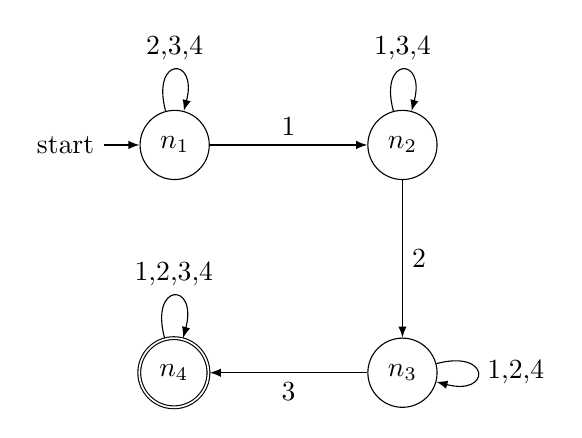
\begin{tikzpicture} [node distance=2cm, auto, every loop/.style={-latex},  every initial by arrow/.style={-latex}]

\node [state, initial] 	(n0){$n_1$};
\node [state] 			(n1) [right=of n0,]	{$n_2$};
\node [state]			(n2) [below=of n1]	{$n_3$};
\node [state, accepting](n3) [left=of n2]	{$n_4$};

\path[-latex] 
		(n0)edge				node	{1}		(n1)
			edge [loop above]	node	{2,3,4}	()
		(n1)edge				node	{2}		(n2)
			edge [loop above]	node	{1,3,4}	()
		(n2)edge				node	{3}		(n3)
			edge [loop right]	node	{1,2,4}	()
		(n3)edge [loop above]	node	{1,2,3,4}()
		;


\end{tikzpicture}
\end{center}
\caption{\label{fig:FSM}A Finite State Machine.}
\end{figure}

\newpage
\section{Phases of the lab}
This lab contains the following steps:

\begin{enumerate}
%\item Create an Android application project in Eclipse.
\item Gather acceleration data for different types of walking. You can look at how phone placement affects the accelerometer data. You could also look at how acceleration data for a running gait differs from a walking gait. (We'll test fast-walk versus slow-walk.)
\item Write an algorithm to eliminate noise from your input.
\item Write an algorithm to detect the gaits you have identified.
%\item Write an algorithm to account for different orientations of the phone.
%\item Integrate and test.
%\item Demonstrate.
\end{enumerate}
%\todo{Should we move the rotation part of this to lab 3?}

\section{Deliverables}
For this lab, your application must display the number of steps the user has taken from a starting position. (See Figure~\ref{fig:lab-2-screen} for an example; you only need to include the number of steps, though.) You must also have a way to reset the count of steps. For full marks, your counter should be accurate to within 10\% of the actual number of steps taken. You may, within reason, ask that the TA evaluating your application carry the phone in a particular way.

\begin{figure}[h]
\begin{center}
\includegraphics[width=0.25\textwidth]{device-screenshot-lab-2.png}
\end{center}
\caption{\label{fig:lab-2-screen}A complete lab 2 implementation.}
\end{figure}

\section{Important Reminders}
\begin{enumerate}
\item Remember to name your project \textbf{Lab2\_SSS\_XX} where SSS is your lab section (e.g. 201) and XX is your team number (e.g. 02). 
\item Different hardware has different levels of noise and bias. Your application should be capable of calibrating itself to new sensors, but this is something to keep in mind.
\end{enumerate}

\section{Demonstration}
Once you are satisfied that your design and implementation are working correctly, arrange a demonstration with a teaching assistant.  You will need to have the TA complete an assessment form.  All of the members of your laboratory group must sign the completed assessment form.  Your grade will be based on the results of the project demonstration at the end of the laboratory session and an evaluation of how well your code follows engineering design principles. (We will run plagiarism detection software on the source code, which may subsequently lower your grade and trigger a Policy 71 case. Don't plagiarize!) You may bring your own device for the demonstration, or you may use load your application onto the device that the teaching team provides.

\paragraph{Requirements}

We will measure your pedometer on 5 walks, each about 20. We'll throw out the worst result. The first four walks will each be at different speeds. The last walk will be at the same speed as the trial in which you had the greatest error. This procedure is intended to protect you from random bugs and user error, but to expose systemic flaws in your implementation.

During testing, you will notice that your pedometer responds to step-like events that are not actually steps. Examples include standing up, rotating the phone, or shaking the phone. You will need to eliminate or significantly reduce at least one of these kinds of false positives:

\begin{itemize}
\item Shaking the phone should not cause steps.
\item Rotating the phone about its axis. (for instance, making a series of short twists around one axis).
\item Moving your hand up and down should not trigger a step.
\item Standing up and sitting down should not trigger a step.
\end{itemize}

The evaluation of this aspect of the lab will be more subjective than the rest of the lab. You will need to explain how you are accounting for these false positives, and your solution should be noticeably less prone to these false positives than a solution that does not implement your improvements.

Recommendation: start by writing an implementation which satisfies all other requirements of the lab but is prone to false positives. Then, improve your solution. To help convince your teaching assistant that you have made significant improvements in accuracy, you should keep your first implementation and display the number of steps it is reporting for comparison. You might want to display both numbers at the same time.

\section{Submission of project files}

Upload the version of your code used in the demo to your subversion repository and commit it. The address is:
\url{https://ecesvn.uwaterloo.ca/courses/ece155/w15/groups/group-NNN-MM}

Email Sanjay Singh if you can't commit to that address.


\end{document}
